\documentclass[11pt,letterpaper]{article}
\usepackage[utf8]{inputenc}
\usepackage[english]{babel}
\usepackage{titlesec}
%%%%%%%%%%%%%%%%%%%%%%%%%%%%%%%%%%%%%%%%%%%%%%%%%%%%%
\usepackage{amsmath}
\usepackage{amsfonts}
\usepackage{amssymb}
\usepackage{mathtools}
\usepackage[margin=1in]{geometry}
\newtheorem{exmp}{Example}
%%%%%%%%%%%%%%%%%%%%%%%%%%%%%%%%%%%%%%%%%%%%%%%%%%%%%
\usepackage{graphicx}
\usepackage{tikz}
\usetikzlibrary{calc}
\usepackage{tikz-3dplot}
%%%%%%%%%%%%%%%%%%%%%%%%%%%%%%%%%%%%%%%%%%%%%%%%%%%%%
\usepackage{varioref}
\usepackage{fancyref}
\usepackage{float}
\floatstyle{boxed}
\restylefloat{figure}
\usepackage{framed}
%%%%%%%%%%%%%%%%%%%%%%%%%%%%%%%%%%%%%%%%%%%%%%%%%%%%%
\usepackage[]{algorithm2e}

\usepackage{listings}
\usepackage{color}

\titleformat{\subsection}[runin]
  {\normalfont\large\bfseries}{\thesubsection}{1em}{}
\titleformat{\subsubsection}[runin]
  {\normalfont\normalsize\bfseries}{\thesubsubsection}{1em}{}

\definecolor{dkgreen}{rgb}{0,0.6,0}
\definecolor{gray}{rgb}{0.5,0.5,0.5}
\definecolor{mauve}{rgb}{0.58,0,0.82}

\lstset{language=Java,
  aboveskip=3mm,
  belowskip=3mm,
  showstringspaces=false,
  columns=flexible,
  basicstyle={\small\ttfamily},
  numbers=none,
  numberstyle=\tiny\color{gray},
  keywordstyle=\color{blue},
  commentstyle=\color{dkgreen},
  stringstyle=\color{mauve},
  breaklines=true,
  breakatwhitespace=true,
  tabsize=3
}
%%%%%%%%%%%%%%%%%%%%%%%%%%%%%%%%%%%%%%%%%%%%%%%%%%%%%
%Script R%
\usepackage{calligra}
\usepackage{qtree}
\DeclareMathAlphabet{\mathcalligra}{T1}{calligra}{m}{n}
\DeclareFontShape{T1}{calligra}{m}{n}{<->s*[2.2]callig15}{}
\newcommand{\scripty}[1]{\ensuremath{\mathcalligra{#1}}}
\newcommand{\sr}{\scripty{r}}
\newcommand{\vsr}{\vec{\sr\,}}
%%%%%%%%%%%%%%%%%%%%%%%%%%%%%%%%%%%%%%%%%%%%%%%%%%%%%
%Macros%
\newcommand{\dint}[2]{\int\limits_{#1}^{#2}}
\newtheorem{ex}{Example}
\newtheorem{thm}{Theorem}
\newtheorem{defn}{Definition}

%%%%%%%%%%%%%%%%%%%%%%%%%%%%%%%%%%%%%%%%%%%%%%%%%%%%%
\author{Alex Pizzuto}
\title{CS 577 Notes}
\begin{document}
\date{}
\maketitle
\hrule

\section{Merge Sort}
The general idea: divide the array into 2 parts, recursively sort by dividing the subarrays into two parts until you reach a certain size and then you merge. 

\begin{algorithm}[ht]
	Declare two pointers\;
	\While{no array is empty}{
	Compare the two numbers pointed to by the two pointers\;
	Add the smaller one to output array\;
	Move the pointer of the array with smaller number to the next element\;}
	Copy all remaining elements in the non-empty array into output array\;
	\caption{Merge Sort}
\end{algorithm}
We can analyze the complexity as follows: 
\begin{equation*}
	T(n) = 2T(n/2) + c n
\end{equation*}
And it is possibly best visualized as a binary tree.
\begin{figure}[h]
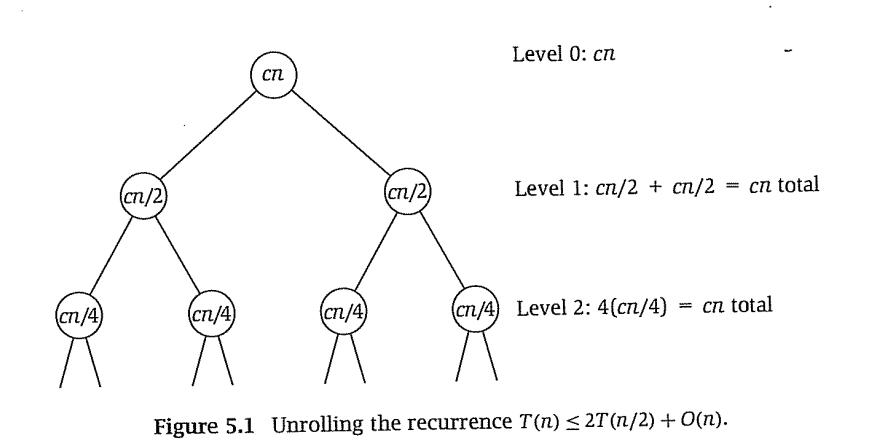
\includegraphics[width=8cm]{MergeTree}
\end{figure}
Working out the complexity a bit more, 
\begin{align*}
	T(n) &= 2T(n/2) + c n \\
	&= 4T(n/4) + 2c n \\
	&= 8T(n/8) + 3cn \\
	& . . . \\
	&= 2^k T(\frac{n}{2^k}) + k c n \;\; \mbox{when} \frac{n}{2^k} = 1 \\
	&= n T(1) + c n \log_2 n \\
	&= c n \log_2 n \Rightarrow \mathcal{O}(n\log_2 n)
\end{align*}
Here the class seemed pretty confused, so we just calculated a few other complexity bounds:
\begin{align*}
	T(n) &= q T(n/2) + cn \\
	&= q^2 T(n/4) + cn + cn \frac{q}{2} \\
	& \vdots \\
	&= c_1 q^{\log_2 n} + c_2 n \frac{(q/2)^{\log_2 n}-1}{(q/2)-1} \\
	&= c_1 n^{\log_2 q} + c_2' n n^{\log_2 q -1} \\
	&\Rightarrow \mathcal{O}(n^{\log_2 q})
\end{align*}
\subsection*{Local Work}
Another helpful methodology of calculating an upper bound includes the notion of the "local work". Take for example 
\begin{equation*}
	T(n) = T(n/2) + T(n/3) + c \cdot n
\end{equation*}
Then at level 0, we make two recursive calls ($n/2$ and $n/3$), but we also do $c\cdot n$ amount of work. Then, we look at the first level of recursive calls. Although the calls make calls, they also do local work (ie $c(n/2 + n/3)$). This continues down the tree, at each level doing $c\cdot n(5/6)^i$ amount of local work. So, 
\begin{align*}
	T(n) &\leq \sum_{i=0}^h(5/6)^i\cdot c n \\
	&\leq 6\cdot cn
\end{align*}
\section{Counting Inversions}
\begin{exmp}
	Suppose you ask somebody for their favorite five movies, and they give you the list: \newline T  S  A  B  E  F \newline 1  2  3  4  5  6  \newline
And then you ask a friend to rank these five movies in their order, and they give you
\newline 4  3  1  5  2  6 \newline
And we are asked how many things are out of order, or how many Inversions there are. 
\end{exmp}
\textit{Inversion}: if $i < j$ but $a_i > a_j$. 
\begin{figure}[ht]
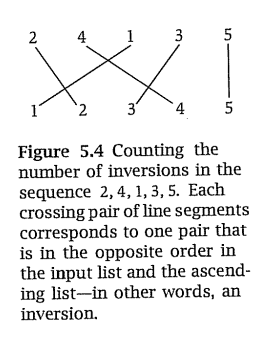
\includegraphics[width=5cm]{InversionCounting}
\end{figure}

\begin{algorithm}[h]
	\If{size = 1} 
	{return\;}
	Divide the array into two halves\;
	Count inverse in left half\;
	Count inverse in right half\;
	Combine the results\;
	\caption{A first try at counting inversions}
\end{algorithm}
But this algorithm yields a result that is $\mathcal{O}(n^2)$. So one way to do it is to sort using a merge sort, and then keep a counter of how many times you have to merge an element into the incorrect side.

\section{Finding the Closest Pair of Points}
Given $n$ points in the plane, find the pair that is closest together. We will show there is an $O(n \log n)$ solution. Assume no two points in $P$ have the same $x$-coordinate or $y$-coordinate. We do it by dividing the plane into two halves recursively. First, sort the $x$-coordinates and the $y$-coordinates in lists $P_x$ and $P_y$, where in each list is a record of where the corresponding element is in the other list. Divide the plane by the median $x$ coordinate ($O(n)$ time). Then we make four lists: $Left_x$, $Left_y$, $Right_x$, $Right_y$. Find the closest pairs now in just the left and right. Then make sure there were no terms crossing the boundary that are closer, by using the minimum distance that you found from the halves as a benchmark. There are at most 15 points in this fuzzy region, and there's a neat geometric proof of this. 

\section{Integer Multiplication}
The traditional multiplication algorithm is quadratic from having to find all of the sub products. The algorithm in the book makes three recursive calls per level making the running time subquadratic
\begin{align*}
	T(n) &\leq 3 T(n/2) + c\cdot n \\
	&\Rightarrow T(n) = \mathcal{O}(n^{\log_2 3}) = \mathcal{O}(n^{1.59})
\end{align*}

\section{June 21 Review Session: Practice Problems}
Suppose you are given an array \texttt{A[1..n]} of sorted integers that has been circularly shifted by an unknown number of spaces, ie \texttt{[5,15,25,35,45,55]}$\to$\texttt{[35,45,55,5,15,25]}. Find max value in $\log n$ time.

Note: In general, when asked to create something that runs in $\log n$ time, a general rule of thumb is that the recurrence relation $T(n) = T(n/2) + c$ runs in $\log n$ time. If asked for $n\log n$, go off the example of Merge Sort, look for $T(n) = 2T(n/2) + O(n)$. 

Back to the problem. 
\begin{algorithm}[ht]
	\eIf{ j-i $\leq$ 2}{return max(A[i], A[j])\;}
	{set k=(i+j)/2\;
	\eIf{A[k+1]<A[k]}{return A[k]\;}{
	\eIf{A[k]>A[j]}{return FindMax(k+1, j)\;}{return FindMax(i, k)\;}}}
	\caption{FindMax(i,j) algorithm for shifted array}
\end{algorithm}
To be rigorous, we should check to make sure that the recursive calls are on circularly shifted arrays still (it is). To verify the running time:
\begin{align*}
T(n) &= T(n/2) + c \\
&\Rightarrow T(n) = \mathcal{O}(\log n)
\end{align*}

The second question asked about finding an $n\log n$ algorithm to check for duplicates. Just do a Merge sort and run through the array once. 

Next we did question 4. describe an algorithm that finds the largest subset of $\mathcal{L}$ , where $\mathcal{L} = a_1, a_2, \ldots , a_n$, whose sum is at most $M$. Run in linear time. Assume we have an algorithm which finds median in linear time to be used as a subroutine. We know that a linear recurrence is something that looks like $T(n) = T(n/2) + c\cdot n$. 
\begin{algorithm}[ht]
	med = FindMedian(L)\;
	lessthanMed = elts in L less than med\;
	greatthanMed = elts in L greater than med\;
	Sum = sum of elts in lessthanMed\;
	\eIf{Sum $\geq$ M}{FindLS(lessthanMed, M)\;}{return size(lessthanMed) + FindLS(greatthanMed, M-Sum)\;}
	\caption{FindLargestSum(L, M) algorithm which outputs size of largest subset of an array L which adds up to less than M}
\end{algorithm}

\section{June 25, 2018}
\begin{defn} 
	\underline{Greedy Algorithm} A type of heuristic algorithm that achieves the optimal solution
\end{defn}
\subsection*{Stay Ahead Method}
\begin{enumerate}
\item \textbf{Define your solutions.} Greedy solutions are typically denoted by ``A", whereas the assumed optimal solution is denoted by ``O".
\item \textbf{Define your measure.} Choose some characteristic of the problem that the algorithm can optimize at each step. This procedure of incremental optimization will inform the algorithm of the next step it needs to take.
\item \textbf{Prove the algorithm ``Stays Ahead".} Usually done via mathematical induction. Goal is to show that your greedy solution is always better or equal to the assumed optimum.
\item \textbf{Prove the optimality.}
\end{enumerate}

\subsection*{Example: Interval Scheduling}
\textbf{Objective:} Schedule the maximum number of classes. Possible heuristic approaches could include giving priority to the earliest start time, shortest duration, earliest end time, etc.\\

\bigskip

Outline of the algorithm: (1) sort the classes based on finishing time. (2) While the list is nonempty, select the first element in the list, remove any tasks in conflict. Note that sorting is $O(n\log n)$ and the while loop is $O(n)$, so in total this approach is $O(n \log n)$.

Step 1: Define solutions \\
A = $\{i_1, i_2, \cdots, i_k \}$ - A particular ordering of $k$ classes, say, an ordering chosen by prioritizing the earliest end time. This solution schedules a maximum of $k$ classes.\\
O = $\{o_1, o_2, \cdots, o_m \}$ - The optimal solution. This ordering will be optimal if $m \geq k$. \\

Step 2: Define the measure \\
Measure = The finish time when $n$ tasks have been completed. We will compare $f(i_n)$ to $f(o_n)$.

Step 3: Prove we ``Stay Ahead"" (Using Induction)\\
\textit{$n=1$}. $f(i_1) \leq f(o_1)$ is obvious since we picked the task with the earliest finishing time. \\
\textit{Assume $f(i_r) \leq f(o_r)$}. $f(i_{r+1}) \geq f(i_r) + t_{r+1}$ where equality would be the case where the classes are scheduled back-to-back. Suppose that we can find a task $o_{r+1}$ such that $f(o_{r+1}) < f(i_{r+1})$. Then this task could also be a candidate solution ''A''. The reason is that\footnote{$s$ denotes the starting time.} $s(o_{r+1}) \geq f(o_r) \geq f(i_r)$, so "A" will choose $o_{r+1}$ instead. Therefore, $f(i_{r+1}) \leq f(o_{r+1})$. \\

Step 4: Prove the optimality, which in this case means we need to prove $k \geq m$.\\
\textit{By contradiction.} Suppose $m > k$. Then there are still tasks after $o_k$ that are compatible with $o_k$. Thus, $s(o_k) > f(o_k) \geq f(i_k)$. But this contradicts the result of step 3: $f(i_k) \leq f(o_k)$, so we have shown that it must be the case that $k \geq m$.


And then we talked about different heuristic methodologies (shortest duration first vs. earliest deadline first) for the optimal class scheduling problem.

\section{Exchange Argument}
Step 1: Label your algorithm's solution (A) and \underline{optimal} solution (O)

Step 2: Compare solutions: Either there is a component in O but not in A or the sequence of tasks in A is different in O

Step 3: Exchange/Swap

Now lets work on an example: Scheduling to Minimize Lateness

We define our greedy solution, $A = \{a_1, a_2,\ldots, a_n\}$ where $d(a_1) < d(a_2) <\ldots<d(a_n)$. We also have $O = \{o_1, o_2,\ldots, o_n\}$. To define a different purposed optimal solution, we must have at least one pair $i, j$ such that $d(o_i) > d(o_j)$ where $i<j$. 

Step 3 now: If there is an inversion, then there must be two neighboring tasks that create an inversion. By exchanging sequence of neighboring tasks of inversion, the maximum lateness will decrease or stay the same. (Looking at an inversion from the optimal solution) For task $o_{i+1}$, its finish time becomes earlier, so its lateness does not go up. Denote $l_i$ as the lateness of task $o_i$ before swap and $\bar{l_i}$ as lateness of $o_i$ after swap. 
$$\bar{l_i} = \bar{f_i} - d_i = f_{i+1}-d_i < f_{i+1} - d_{i+1} = l_{i+1}$$
Thus, we have $\bar{l_{i+1}} < l_{i+1}$. 

Step 4: Iterate: In $O$, we have at most $\frac{n(n-1)}{1}$ inversions. After completing all inversions, $O$ became $A$, and he maximum lateness does not increase. This means that solution $A$ is at least as good as solution $O$, thus the greedy solution is the optimal solution. 

\section{June 25, 2018 Review Session Notes}
\subsection*{Example: Truck Packing}
You are consulting for a trucking company that loads packages $i$ with weigths $w_i$ in the order received until they can't fit any more boxes in a truck (meets threshold $W$). Prove to them that their greedy algorithm is the best method possible.
 
Solution: A set $\{ i_1, i_2, \ldots, i_k \}$ where $i_r$ denotes the last package shipped in truck $r$. Let $S$ denote the solution obtained by the "greedy" procedure, $S = \{ i_1, \ldots, i_m\}$, and we aim to show that for any other solution $O = \{ j_1, \ldots, j_k \}$, we have $m \leq k$. 

\textbf{Proof}: Greedy "Stays Ahead"

Claim: $\forall r \geq 1$, we have $i_r \geq j_r$. \textit{Proof by Induction} \textbf{Base case}: $r = 1$. By definition, we have $i_1 \geq j_1$ because by construction we put in as many packages as possible, so if $j_1 > i_1$, then $\sum_{l=1}^{j_1}w(l) > W$, which we cannot have. 

\textbf{Inductive step}: Assume $i_{r-1} \geq j_{r-1}$ for some $r \geq 1$. We will prove that $i_{r} \geq j_{r}$. Suppose (for contradiction) $i_r < j_r$. Then the packages shipped in truck $r$ of solution $O$ are $\{ j_{r-1}+1,\ldots,j_r \}$. Since $i_{r-1} \geq j_{r-1}$, then the set shipped by the optimal solution contains $\{ i_{r-1} + 1,\ldots, i_r + 1\}$, but this goes against the construction of our greedy set, and thus the optimal solution would have a truck that exceeds the weight limit. Thus $i_r \geq j_r$. QED. 

To complete the proof, we show that $|S| \leq |O|$. Suppose this is not true. Then let $k$ be the size of $O$. By claim, $i_k \geq j_k$, thus there are packages that are not shipped by the optimal solution, and our greedy solution is the best solution. 

\subsection*{Example: Houses Along a Highway}
Suppose we have $n$ houses distributed along the highway at locations $\{x_1, \ldots, x_n\}$, and we seek to distribute cell towers (with a 4 mile range) along the path with as few cell towers as possible so that all houses are covered. Our solution: While there are uncovered houses, pick the leftmost uncovered house, and put a cell tower 4 miles to the right of said house. Let $S = \{ t_1, \ldots, t_k\}$ be the solution obtained by the greedy algorithm. Let $O = \{s_1,\ldots, s_m\}$ be a purported optimal solution. We seek to prove that $|S| \leq |O|$. Assume tower locations are listed left to right. Claim: $\forall r>0$, we have $t_r \geq s_r$ (proof left to the reader).

\textbf{Proof}: By Induction

Suppose that this is not true (ie suppose $k > m$). By the claim, $t_m \geq s_m$. There are no towers to the right of $s_m$ in $O$, but there are houses not covered by $t_m$, meaning not all houses would be covered by $O$. QED. 

\section*{Graphs (June 26, 2018)}
\begin{defn}
	We define a \underline{Graph} $G = (V, E)$ as a set of vertices, $V$, and edges, $E$ connecting said vertices (possibly with weighting)
\end{defn}
Some terminology that accompanies this definition:
\begin{itemize}
	\item \underline{path}: consecutive edges that connect two vertices
	\item \underline{cycle}: A path that starts and ends at the same vertex
	\item \underline{vertex degree}: Number of edges coming out of a vertex
\end{itemize}
One of the many theorem's of Euler: If you have a node with an odd vertex degree, you can't have a cyclic path that traverses all edges. 

TSP: Hamiltonian cycle is kind of a ubiquitous problem in CS. 

Node traversals and cycle detection: Breadth First Search. 
Pick one vertex out of $E$, add it to $L_0$. Declare $i$ as a layer number, initialize to 0. While there are still vertices in $L_i$ not checked, randomly select one vertex $u$. For all vertices $v$ not in $L_0,\ldots,\L_i$, if there is an edge $u\to v$, add $v$ to $L_{i+1}$. Mark $u$ as being visited. 

\subsection*{Shortest Path Problem}
Dijkstra's Algorithm

\section*{Review Session: June 26, 2018}
Assume you have been given two sets $r_1,\ldots,r_n$ and $c_1,\ldots,c_n$ and we seek to create a matrix with entries either equal to 1 or 0 such that the sum of the $i^{th}$ row is equal to $r_i$ and the sum of the $j^{th}$ column is equal to $c_j$. As an example, with $r = \{ 1, 2, 4, 4\}$ and $c = \{2, 3, 3, 3\}$ we could have 
\[\begin{pmatrix} 0 & 1 & 0 & 0 \\
0 & 0&1&1& \\
1&1&1&1\\
1&1&1&1
\end{pmatrix}
\]

We have defined the greedy algorithm as follows. In the $i^{th}$ row, distribute $r_i$ ones based off of a max priority queue from the remaining entries needed for the $c_j$.

\section*{Minimum Spanning Problem (June 28, 2018)}
Given a set of nodes, $V$, we seek to construct a connected graph that has the minimum number of total edge cost.

The resulting graph is a tree.

\textbf{Proof}: Suppose there is an optimal solution of connected graph that is not a tree. Then this graph has at least one cycle, $C$. If we delete an edge $e \in C$, the graph is still connected, but the result is $l_e$ less. 

First attempt at finding tree: (\textit{Reverse Delete Algorithm}) Take away the longest edge only if it does not result in a disconnected graph

Second attempt: (\textit{Kruskal's Algorithm}) Add edges with minimum length so far only if it does not create a cycle

Third attempt: Start with the root node, select the edge with the maximum length. Use the newly added node as the starting node. Repeat the process for choosing the node with minimum edge cost to this node, but does not create a cycle. This one doesn't work, btw

Fourth attempt: (\textit{Prim's Algorithm}) Start with the root node, add it to the explored set $S$. 
\begin{algorithm}
	\While{$S \neq V$}{
	\For{all nodes u in $S$}{
	Check all nodes $v$ in $V-S$\;
	Select node $v$ such that it is the minimum edge cost\;
	Add $v$ into $S$}}
	\caption{Another attempt at this problem}
\end{algorithm}

Now, let's prove that \textit{Kruskal's} and \textit{Prim's} actually work. Before doing that, a quick definition.
\begin{defn}
	\underline{Cut Property}: Let $S \subset V$ and $S \neq \{\}$, let $e = (u,v)$ be the minimum cost edge with $u \in S$, and $v \in V-S$. Then, the minimum spanning tree, $T$, must include $e$.
\end{defn}
\textbf{Proof}: By Exchange Argument. Assume there exists a distinct optimal solution from our supposed solution. So that means we have a different edge, $e' = (u', v')$ connecting $S$ and $V-S$. Since $T$ is a spanning tree, there must be a path from $u\to u' \to v' \to v$. If we exchange $e$ for $e'$ (ie replace $e'$ with $e$), the resulting cost will be $$T-l_{u', v'} + l_{u,v} < T\; .$$ After the exchange of $e$ for $e'$, the graph still stays connected because any previous path going through $u' \to v'$ can be rerouted as $u'\to u\to v\to v'$. 

\textbf{Proof}: of \textit{Kruskal's Algorithm}. We seek to prove that this algorithm results in a \underline{MST} (Minimum Spanning Tree). Let $S$ denote the graph where node $u$ has a path to all nodes in it. This means $u \in S$, but $v \notin S$. Otherwise edge $(u,v)$ will create a cycle. Since $l_{u,v}$ is the cheapest edge in the remaining set of edges, based on the cut property, it must be included in the MST. Next, we prove that Kruskal's algorithm results in a tree. Thus, we must show that the graph is connected and does not contain a cycle. The algorithm forbids adding edges which would result in a cycle, thus we know that there are no cycles. It's also not too hard to show connectedness. 

\textbf{Proof} of \textit{Prim's Algorithm}: We know that $S$ is always connected, and we iterate until we have included all of $V$. Thus it is clear the graph is connected. And the algorithm prevents cycles. The graph is a partial tree at each level, so we good. 

\begin{defn}
	\underline{Cycle Property}: Let $c$ be and cycle in $G$. Let edge $e = (u, v)$ be the most expensive edge on $c$. Then $e$ does nor belong to the MST.
\end{defn}
\textbf{Proof}: Suppose there exists a distinct optimal solution, and in such a solution there is an edge, $e$, that was the largest edge in a cycle. If we exchange another edge, $e'$, on this cycle for this edge, the resulting cost is $T - l_{e} + l_{e'} < T$. Eventually we can prove that the greedy algorithm Reverse Delete results in lower cost. We have shown before that the graph will still be connected. 

We must still analyze the complexity of these algorithms. For \textit{Prim's Algorithm}, we have $n$ loops, each iteration of the loop can check $m$ things, so the computing complexity is $T(n) = \mathcal{O}(m\cdot n)$. It is worth noting that there is an algorithm that goes like $\mathcal{O}(m \log n)$ if we use the imporved version of Djikstra's algorithm. 

\subsubsection*{Dijkstra's Algorithm: Improved version}
Let $S$ be the explored set of nodes ($S = \{\}$ initially). Initialize $d(s) = 0$ and $d(u) = \infty$ if $u \neq s$. While $S \neq V$, find the $\mu \in V-S$ such that $d(\mu)$ is the minimum. Add $\mu$ to $S$. For all nodes $\nu$ in $V-S$ that is incident to $\mu$, update $d(\nu) \to d(\nu) = min(d(\nu), d(u) + l_{\mu, \nu})$. If you put in a special data structure, ie a priority queue/heap for the inner workings of the loop, then we can achieve $\mathcal{O}(m \log n)$.

\section{July 2, 2018}


\subsection*{Prim's Algorithm}
We looked at Prim's algorithm again at the beginning of the class to analyze the computing complexity

\begin{algorithm}[H]
	Let $S$ denote the explored set, $S = \{ \}$\;
	Let key(u) denote the shortest edge value into u\;
	Let r be the root node, key(r) = 0, key(u) = $\infty$\;
	\While{$S \neq V - \mathcal{O}(n)$}{Select node $\mu$ from $V-S$ such that key is minimum \;
	Add $\mu$ to $S$\;
	for each $\nu \in V - S$, that is a neighbor of $\mu$, update key($\nu$) as min(key($\nu$), $l_{\mu, \nu}$)}
\end{algorithm}

\renewcommand{\arraystretch}{1.5}
\begin{tabular}{ r |c | c | c} \hline
& Unsorted Array & Sorted Array & Binary Heap based prior. queue \\ \hline \hline
Search & $\mathcal{O}(n)$ & $\mathcal{O}(\log n)$ & $\mathcal{O}(\log n)$ \\ \hline
Add & $\mathcal{O}(1)$ & $\mathcal{O}(n)$ & $\mathcal{O}(\log n)$ \\ \hline
Delete & $\mathcal{O}(n)$ & $\mathcal{O}(n)$ & $\mathcal{O}(\log n)$ \\ \hline
\end{tabular}

\section{Dynamic Programming (optimization)}
Weighted Interval Scheduling: Let's suppose that all tasks are marked in the order of finish time. Denote $P(j)$ as the task with the latest finish time ahead of task $j$ but no conflict. We will use $opt(j)$ to denote the optimal cost for scheduling tasks $1, 2, \ldots, j$. Then we have $opt(j) = v_j + opt(p(j))$, if $j$ is scheduled. If $j$ is not scheduled, then we have $opt(j) = opt(j-1)$. This is just an example of a \textit{Binary Choice}. So to do the scheduling, we just find $$opt(j) = \max ( opt(j-1), v_j + opt(p(j)))$$. This is an example of needing to use \textit{Memoization}. 

\begin{algorithm}[H]
	Iterative-opt \\
	Declare M[0...n], M[0] = 0\;
	\For{$j$ from 1 to $n$}{
	M[$j$] = max ( M[$j$], $v_j + $ M[$p(j)$])\;
	}
	Return M[$n$]\;
\end{algorithm}

\textbf{Dynamic Programming Problems:}
\begin{itemize}
	\item The problem can be divided into subproblems
	\item The final problem can be solved relatively easily using the results of the subproblems (subproblem size will be from smallest to largest)
\end{itemize}

Example Problem: Least Squares programming. Assume we seek a regression for a set of points $P$, where $P = {p_1, \ldots, p_n}, \; p_i = (x_i, y_i)$. We know we can represent the regression as $y = a x + b$. We do this by finding the least squares regression:
\[
Error(L,P) = \sum_{i=1}^n (y_i - ax_i -b)^2
\]
Then in order to find the minimum, we optimize:
\begin{align*}
\frac{\partial E(L,P)}{\partial a} &= 0 \\
\frac{\partial E(L,P)}{\partial b} &= 0
\end{align*}

This reduces to 
\begin{align*}
	a &= \frac{n\sum_{i=1}^n x_i y_i - \sum_{i=1}^n x_i \sum_{i=1}^n y_i}{n \sum_{i=1}^nx_i^2 - (\sum_{i=1}^n x_i)2} \\
	b &= \frac{\sum_{i=1}^n y_i - a \sum_{i=1}^n x_i}{n}
\end{align*}

An easier way to do this might be to segment our plane, and then find line segments that optimize subsets of our data (almost like linear splining). 
\begin{itemize}
	\item Idea 1: simply add errors of all segments
	\item Idea 2: Add cost for using more segments for match (call it $c$)
\end{itemize}

$opt(j)$ denotes the optimal total cost for matching nodes $1, 2, \ldots, j$. $e_{i,j}$ denotes the line used to match nodes $i, i+1, \ldots, j$. Then we have:
$$opt(j) = \min(c + e_{i,j} + opt(i-1))$$
With this, we can write out our algorithm:

\begin{algorithm}[H]
	\textbf{Segmented-Least-Squares(P,C)} \\
	M[0,...,n] - minimum cost over nodes $1,\ldots,j$\;
	M[0] = 0\;
	(To compute all possible $e_{i,j}$) \\ 
	\For{$i$ from 1 to $n$}{
	\For{$j$ from $i+1$ to $n$}{
	Compute $e_{i,j}$ using $E(L,P)$ formula and values of $a,b$ computed\;
	}}
	\For{$j$ from 1 to $n$}{
	$M[j] = \min ( c + e_{i,j} + M[i-1])$\;}
	Return M[$n$]
\end{algorithm}
The first set of loops sets the computing complexity of this algorithm to be $\mathcal{O}(n^3)$ assuming that the optimization step is linear in $n$. 

\section{July 9, 2018}
\textbf{Problem: Sequence Alignment}: First we start with a few definitions:
\begin{itemize}
	\item \textit{Matching}: a set of ordered pairs with each item occurring in at most one pair
	\item \textit{Alignment}: is a matching that has no "crossing" pairs. i.e. if $(i,j) \in M$, $(i', j') \in M'$, and $i<i'$ then $j<j'$.
\end{itemize}

We also talked about space-efficient alignment.

\section{Network Flow}
We started talking about Network flow, it looks like we did 7.1-7.3 and 7.5-. Most important result was 7.9: \textit{Let $f$ be a flow s.t. there is no $s\rightarrow t$ path in $G_f$. Let A* be the set of nodes where where is a $s\rightarrow v$ path for $v\in A$*, and no $s\rightarrow w$ path for $w\in B$*} 
$$v(f) = f^{(out)}(A*) - f^{(in)}(A*)$$

7.11: Given a flow $f$ of maximum value, we can compute an $s-t$ cut of minimum capacity in $\mathcal{O}(m)$ time. 


\section{Review for Final}
\subsection*{Greedy Algorithms}
\begin{itemize}
	\item Greedy Stays Ahead
	\item Exchange argument
\end{itemize}

For Greedy Stays Ahead: Define your solution, find the measure, prove greedy stays ahead, prove optimality.

For example, in the gas stations problem, we define our solution, $A$, and seek to prove that given a different optimal solution, $O$, we have $a_i \geq o_i$.

In general, exchange argument works well if you have some sort of sequence sorting. For the exchange argument proff structure: Define your solution, find possible differences (between the greedy and optimal), exchange arguments in the optimal solution, and prove that it becomes closer to the greedy solution, then iterate over all possible changes.

Contiguous subsequence problem. 


\end{document}